\documentclass{article}
\usepackage[utf8]{inputenc}
\usepackage[spanish]{babel}
\usepackage{graphicx, graphics, float, fancyhdr, titling}
\usepackage{listings}
\usepackage[a4paper, total={6in, 9.5in}]{geometry}
\usepackage{fancyhdr}
\usepackage{hyperref}   %para que funcione addcontentsline debe ser la ultima que se cargue

%\setcounter{secnumdepth}{-2}       %Poner solo esto si no se quieren numero delante de las secciones y niveles inferiores.

\renewcommand{\footrulewidth}{0.4pt}
\title{

\includegraphics[width=1.75in]{imagenes/UGR-Logo.png} \\
\vspace*{1in}
\textbf{Cuestiones Tema 2} \\
Animación por Ordenador \\
\vspace*{0.5in}}
\author{Andrés Merlo Trujillo \\
andresmerlo@correo.ugr.es \\
77147239H \\ 
\vspace*{0.5in} \\
E.T.S. de Ingenierías Informática y de Telecomunicación \\
\textbf{Universidad de Granada}} \date{\today}

\hypersetup{
    colorlinks=true,
    linkcolor=black,
}

\renewcommand\maketitlehooka{\null\mbox{}\vfill}
\renewcommand\maketitlehookd{\vfill\null}

\begin{document}
\begin{titlingpage}
\maketitle
\end{titlingpage}

\tableofcontents

\newpage

\pagestyle{fancy}   %a partir de comienza el header (se salta el indice y portada)
\fancyhead[L]{Andrés Merlo Trujillo}
\fancyhead[R]{Animación por Ordenador}
%\section{Ejercicio 1}
%\begin{figure}[H]
%    \centering
%    \includegraphics[width=\textwidth]{imagenes/passwdfile.png}
%\end{figure}

\section{Busca el resto de principios de animación, descríbelos brevemente e indica un ejemplo visual de cada uno.}

Voy a explicar cada uno de los principios en subsecciones a continuación.

% overlap: meh
% slow: arreglar forma en que se dicen las cosas (esta muy raro escrito)
\subsection{Overlap \& Follow Through}

Son dos técnicas que se utilizan con el objetivo de crear una animación más realista y para dar la sensación de que el personaje tiene una inercia [https://www.brownbagfilms.com/labs/entry/12-principles-of-animation-follow-through-and-overlapping-action-tutorials]. La idea principal de estas técnicas las partes secundarias de un personaje se mueven a un ritmo diferente del personaje durante el movimiento del mismo y mantienen una inercia cuando el personjae se para.

\bigskip

\textit{Follow Through} se basa en la idea en que ciertas partes conectadas a un personaje/objeto se seguirán moviendo después de que dicho objeto haya parado [https://www.brownbagfilms.com/labs/entry/12-principles-of-animation-follow-through-and-overlapping-action-tutorials].

\bigskip

Mientras que el \textit{Overlapping} se basa en la idea en que las partes conectadas a un personaje/objeto se moverán a un ritmo diferente del mismo [https://www.brownbagfilms.com/labs/entry/12-principles-of-animation-follow-through-and-overlapping-action-tutorials], normalmente en el sentido contrario en el que se mueven el personaje, para dar sensación de velocidad.

\bigskip

Ejemplos de este principio pueden ser: movimientos de brazos de un personaje, movimiento de las orejas de un animal que correo y luego para, o incluso el movimiento de una antena de un personaje.

\begin{figure}[H]
    \centering
    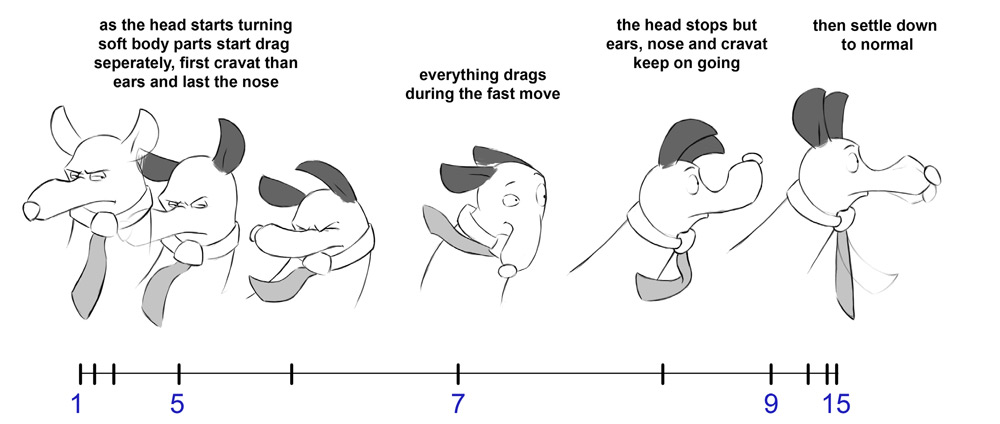
\includegraphics[width=\textwidth]{imagenes/overlap-08.jpg}
    \caption{Ejemplo del principio de \textit{Overlapping} y \textit{Follow Through}. Se puede ver en las orejas y la corbata.}
    \caption{Enalce: https://www.robert-kuczera.de/3d-character-animation-tutorial-secondary-actoin.html}
\end{figure}

\subsection{Slow-in \& Slow-out}

% Este principio consiste en que los objetos cuando se mueven en la vida real no lo hacen de manera abrupta, sino acelerando para comenzar a moverse y decelerando cuando se van a parar. 

Este principio consiste en hacer que un objeto acelere cuando vaya a comenzar a moverse y decelere cuando se vaya a parar. Esto se hace de esta forma porque en la vida real los objetos no se mueven sin antes acelerar o decelerar. Realizar una animación sin este principio puede hacer que los movimientos parezcan naturales, robóticos y abruptos. [https://www.pluralsight.com/blog/film-games/understanding-12-principles-animation]

\bigskip

Un ejemplo de este principio es en un coche que sale de parado y luego frena de nuevo, el coche necesita un tiempo para llegar a la velocidad deseada; es decir, una aceleracion. Luego cuando frena pasa exactamente lo mismo, no para bruscamente, sino que va decelerando poco a poco. [https://www.pluralsight.com/blog/film-games/understanding-12-principles-animation]

\bigskip

En animación tradicional, esto se realiza haciendo uso de espaciados: en el comienzo y final de la animación se dibujan más fotogramas seguidos, mientras que en el resto se mantiene un espaciado mayor, pero constante, para que el resultado final sea el correcto [https://www.pluralsight.com/blog/film-games/understanding-12-principles-animation]. El espaciado menor producirá que se le dedique más tiempo (fotogramas) a la animación, mientras que el mayor menos, haciendo que se de dicha sensación.

\bigskip

En la animación por ordenador, normalmente se suele hacer con una curva \textit{Ease-In/Ease-Out}, que realiza exactamente lo mismo que con las aniamciones tradicionales, pero automaticamente.

\begin{figure}[H]
    \centering
    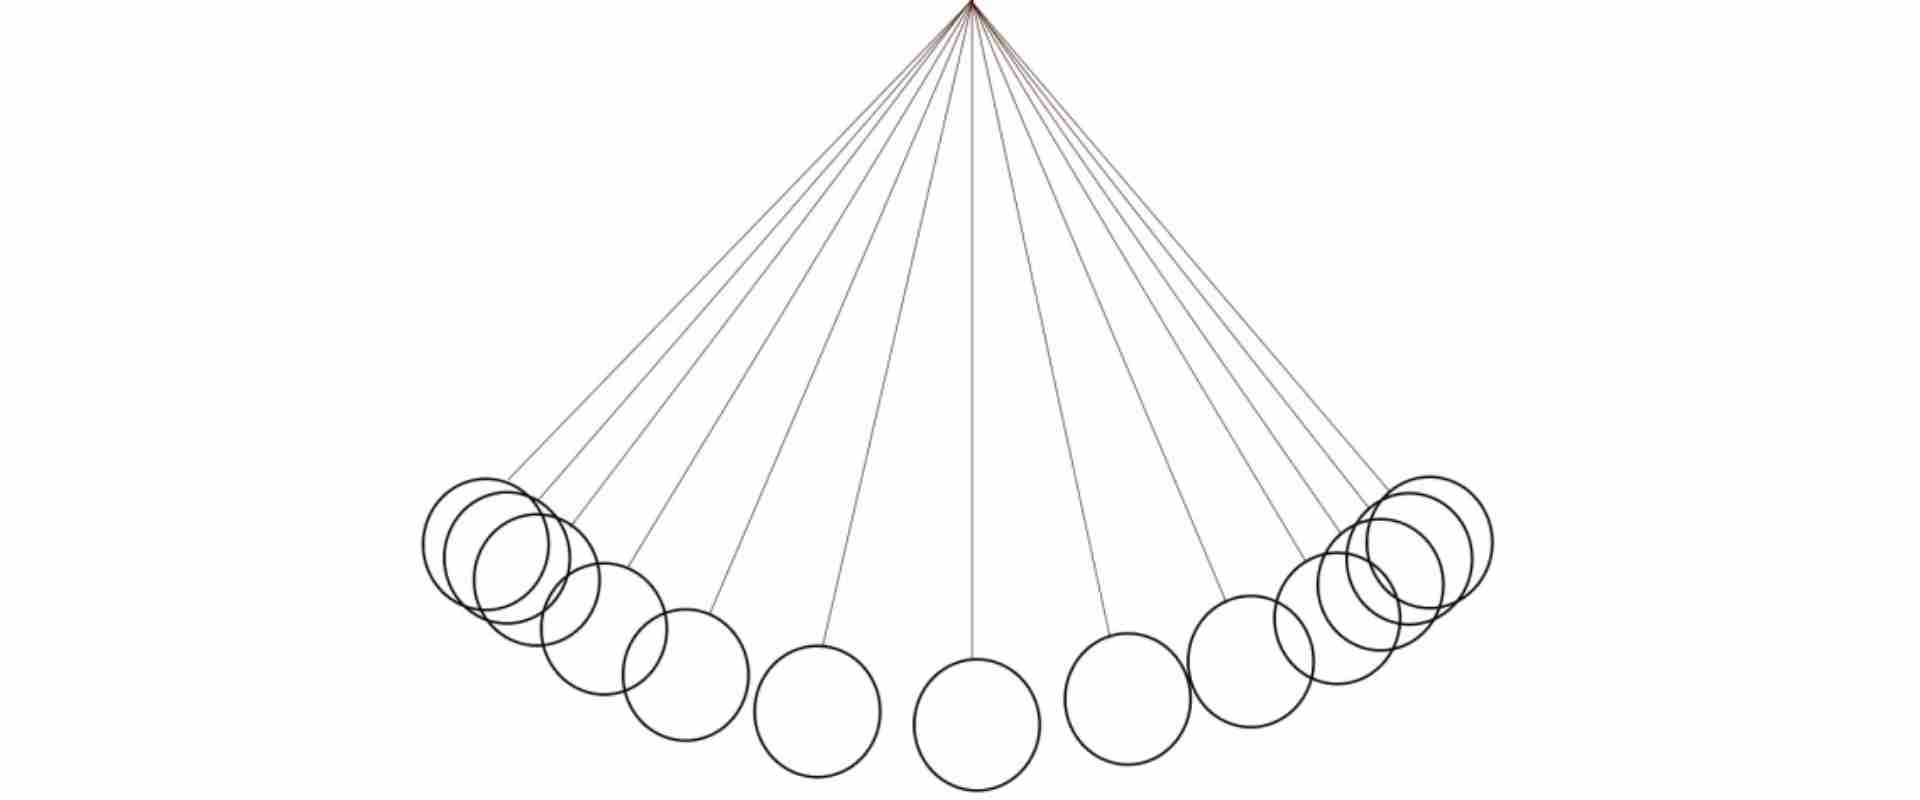
\includegraphics[width=\textwidth]{imagenes/Slow-In-and-Slow-Out.jpg}
    \caption{Ejemplo del principio \textit{Slow-In \& Slow-Out}. Se puede ver como el péndulo en los extremos acelera y decelera mediante el espaciado de los fotogramas.}
    \caption{Enalce: https://darvideo.tv/dictionary/slow-in-slow-out/}
\end{figure}

\subsection{Arcos}

En la vida real, gran parte de los movimientos y acciones que se producen suelen seguir una trayectoria circular, denominada arco [https://dsource.in/course/principles-animation/arcs]. Estos arcos se pueden producir porque incide mas de una fuerza en el objeto, haciendo que este se mueva trazando un arco [https://es.linkedin.com/learning/fundamentos-de-la-animacion/arcos-de-la-animacion]. Otro motivo es porque existen objetos que poseen un pivote (como un brazo), haciendo que el movimiento que realicen se restrinja al arco.

\bigskip

Utilizar arcos hace que la animación sea más natural y fluida, haciendo que sea más creíble para el espectador. Si no se aplicase este principio, la animación sería demasiado mecanizada y robótica.

\bigskip

Algunos ejemplos que se pueden beneficiar de los arcos son: rebote de una pelota, movimiento de una extremidad de un personaje y el movimiento de una rama por el viento.

\begin{figure}[H]
    \centering
    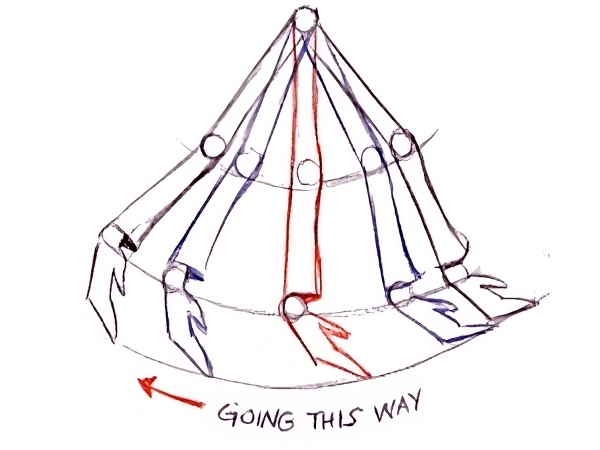
\includegraphics[width=\textwidth]{imagenes/arm-arc.jpg}
    \caption{Ejemplo del principio Arcos. Se puede ver como el movimiento del brazo sigue un arco.}
    \caption{Enalce: https://johnhannonblog.wordpress.com/2015/12/01/12-principles-of-animation-arc/}
\end{figure}

\begin{figure}[H]
    \centering
    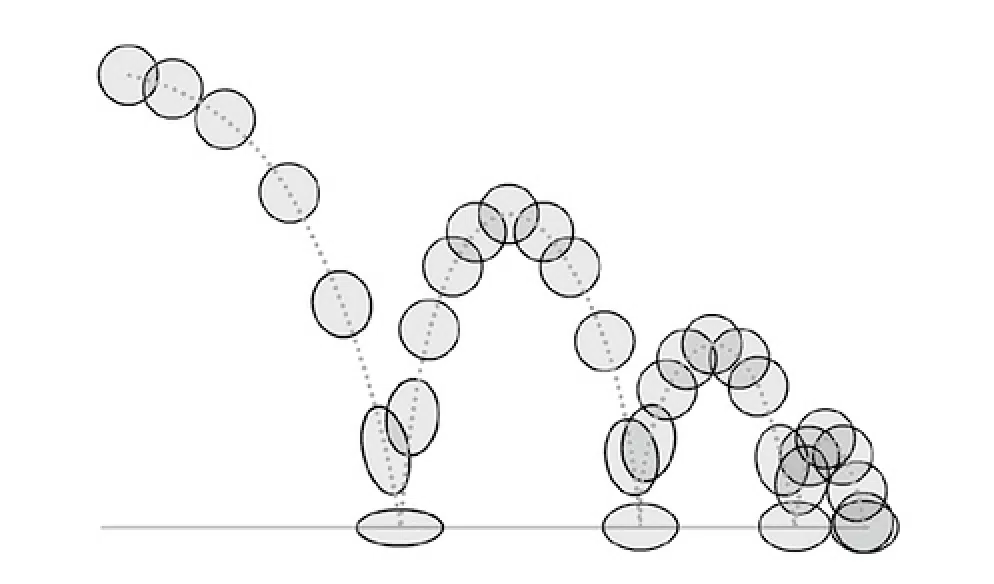
\includegraphics[width=\textwidth]{imagenes/bouncing-ball.png}
    \caption{Otro ejemplo de Arcos. La fuerza de la gravedad y la fuerza de lanzamiento hacen que cree un arco.}
    \caption{Enalce: https://idearocketanimation.com/13721-12-principles-of-animation-gifs/}
\end{figure}

\subsection{Acción secundaria}

Consiste en las acciones que enfatizan la accion principal para darle mas vida a la animacion y hacer que las acciones del personaje sean mas convincentes. Debe ser algo sutil, que no distraiga o tape la accion principal, ya que solo debe aportar mas expresividad a la principal. [https://www.pluralsight.com/blog/film-games/understanding-12-principles-animation]

\bigskip

Además, permite mostrar de manera subconsciente lo que el personaje está pensando [https://idearocketanimation.com/13721-12-principles-of-animation-gifs/], como su estado de ánimo.

\bigskip

Un ejemplo de esto es alguien esperando (acción principal) en una sala de espera, si se le añade la acción secundaria de estar dadndo toques con el pie repetidamente, se percibe la sensación de que está esperando nervioso.

\begin{figure}[H]
    \centering
    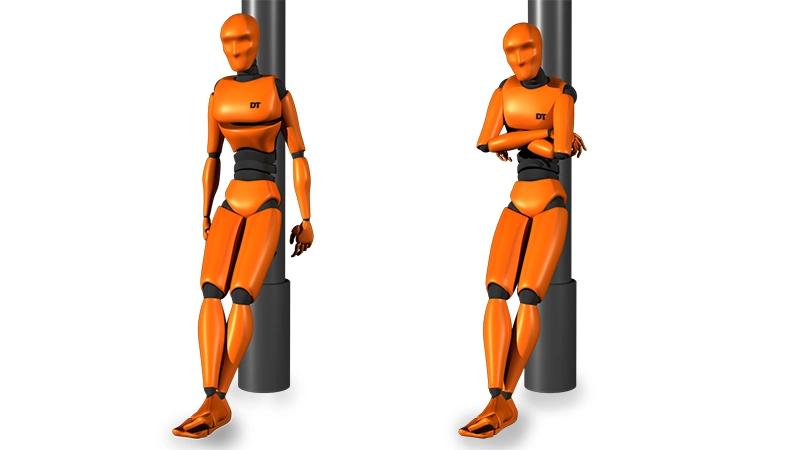
\includegraphics[width=\textwidth]{imagenes/secondary-action.png}
    \caption{Ejemplo de acción secundaria. Se puede ver que puede transmitir otra sensación la posición de los brazos.}
    \caption{Enalce: https://www.pluralsight.com/blog/film-games/understanding-12-principles-animation}
\end{figure}


\begin{figure}[H]
    \centering
    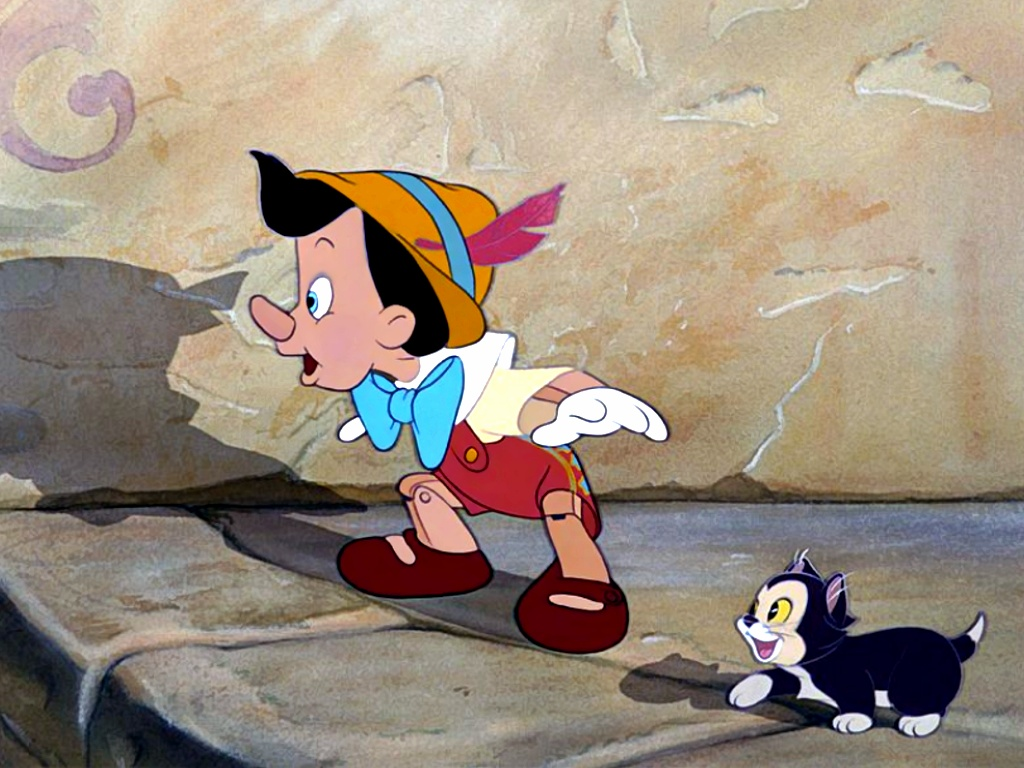
\includegraphics[width=\textwidth]{imagenes/sec-ac.jpg}
    \caption{Otro ejemplo de acción secundaria. Se puede ver que la expresión facial se complementa con los brazos levantados.}
    \caption{Enalce: https://animation2012.weebly.com/secondary-action.html}
\end{figure}
\subsection{Timing}

Consiste en como distribuir los fotogramas de una acción; es decir, en cuantos fotogramas se debe realizar una acción [https://idearocketanimation.com/13721-12-principles-of-animation-gifs/].

\bigskip

El \textit{timing} se puede aplicar a velocidad de movimientos o la duración de los fotogramas. Ajustando el \textit{timing}, se puede expresar que un personaje es más ágil o pesado, más rápido o más lento, etc. También permite mostrar sitaciones de nerviosismo, comeddia, etc.

\bigskip

Un ejemplo de esto puede ser para escenas en películas de acción, donde el personaje necesita actuar rápido para poder alcanzar un objetivo. En este caso lo mejor es usar un timing más espaciado, haciendo menos fotogramas para dar la sensación de rapidez en la escena. 
%dejado intencionadamente asi
Otro ejemplo puede ser el de un espectador en una pista de carreras observando los coches, estos deben tener pocos fotogramas para dar la sensación de que va muy rápido.

\begin{figure}[H]
    \centering
    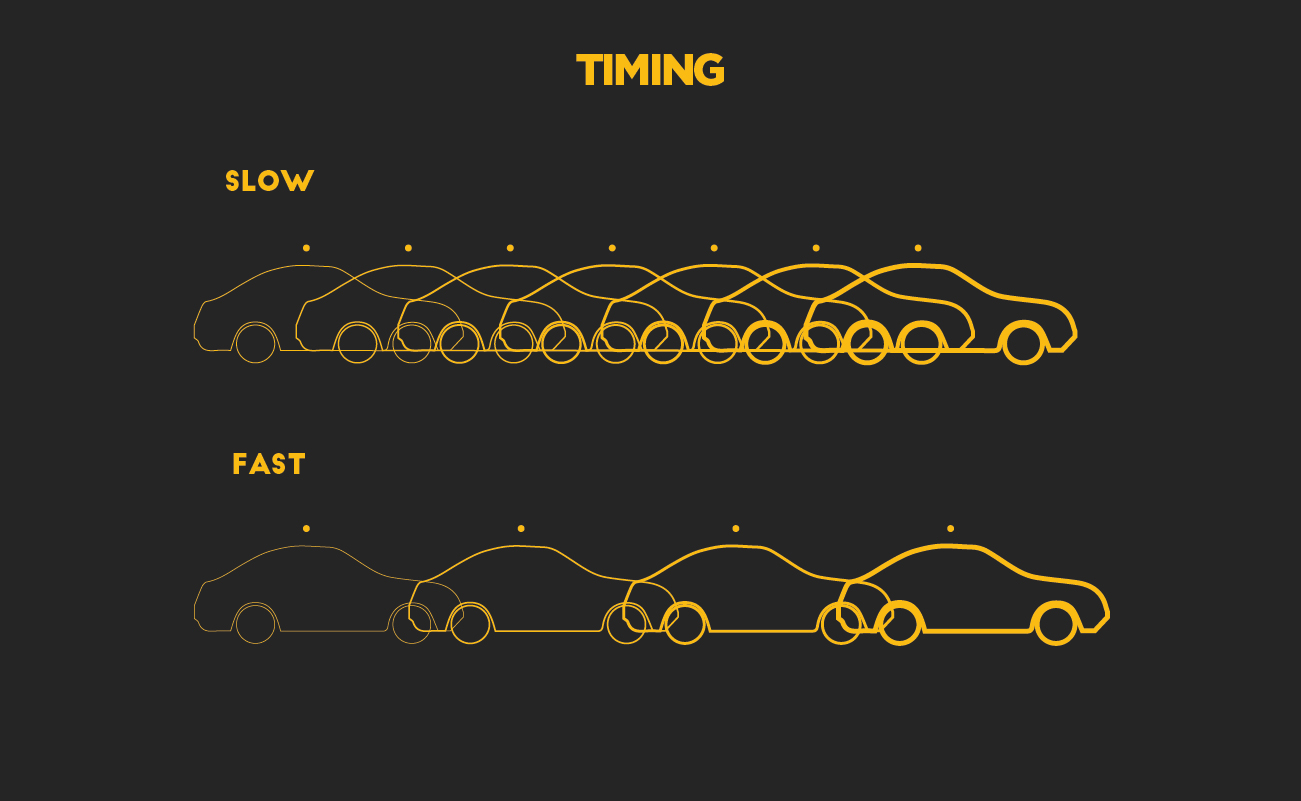
\includegraphics[width=\textwidth]{imagenes/image-9_timing.jpg}
    \caption{Ejemplo de \textit{timing}.}
    \caption{Enalce: https://www.360south.com.au/blog/article/27/the-12-principles-of-animation-part-three.html}
\end{figure}

\subsection{Exageración}

Consiste en exagerar los movimientos, emociones y acciones de los personajes con el objetivo de que la animación sea más humorística, emocionante o dramática.

\bigskip

Un ejemplo clásico es el de un personaje sorprendido, ya que normalmente los animadores lo dibujan con los ojos mucho más abiertos de lo normal (e incluso en algunos casos se puedan salir) y su boca se abra de par en par.

\begin{figure}[H]
    \centering
    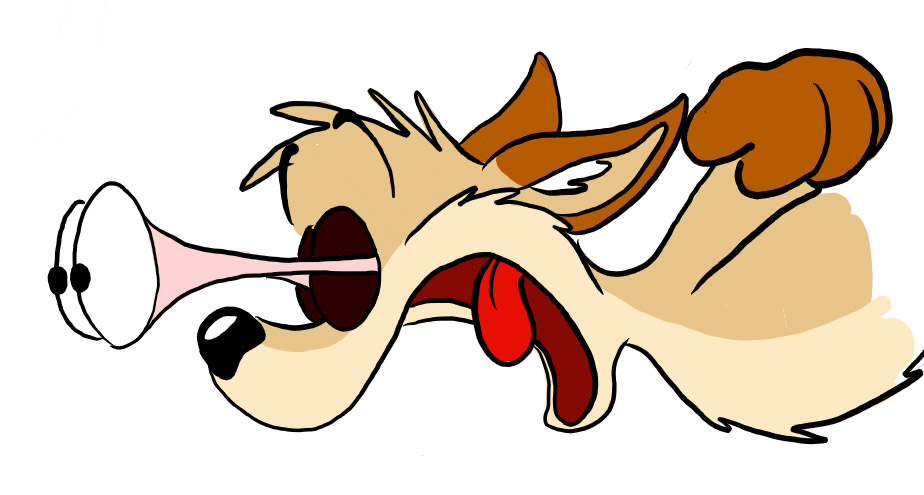
\includegraphics[width=\textwidth]{imagenes/080104_eyes.jpg}
    \caption{Ejemplo de exageracion.}
    \caption{Enalce: https://nutchelleblog.wordpress.com/2015/11/22/exaggeration/}
\end{figure}

\begin{figure}[H]
    \centering
    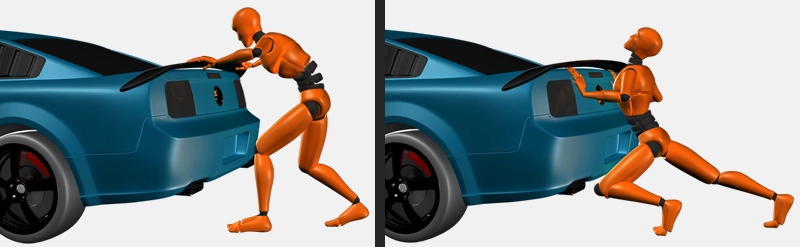
\includegraphics[width=\textwidth]{imagenes/Exaggeration.png}
    \caption{Otro ejemplo de exageracion mas realista.}
    \caption{Enalce: https://www.pluralsight.com/blog/film-games/understanding-12-principles-animation}
\end{figure}

\subsection{Poses sólidas}

Se refiere a la habilidad de crear dibujos tridimensionales que tengan una sensaci'on de peso, profundidad y volumen correctos y convicentes [https://www.pluralsight.com/blog/film-games/understanding-12-principles-animation].

\bigskip

Es esencial que los animadores tengan una clara comprensión del espacio tridimensional y perspectivas de todos los ángulos de los personajes para poder ubicar los objetos de manera correcta en el espacio y tenga la escena sensación de profundidad.

\bigskip

Otro aspecto importante de las poses sólidas es el de evitar \textit{twinning}, que como se dijo en clase, consiste en evitar poner cualquier par de extremidades simétricas, ya que resulta muy forzado y rígido [https://www.pluralsight.com/blog/film-games/understanding-12-principles-animation].

\begin{figure}[H]
    \centering
    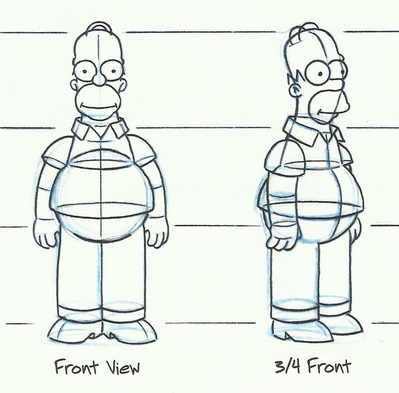
\includegraphics[width=\textwidth]{imagenes/homer-solid-drawing.jpg}
    \caption{Ejemplo de poses sólidas. Aparece Homer en diferentes perspectivas correctamente. También es un buen ejemplo de \textit{twinning}, es demasiado rígido al ser simétrico.}
    \caption{Enalce: https://johnhannonblog.wordpress.com/2015/12/01/12-principles-of-animation-solid-drawing/}
\end{figure}

\subsection{Personalidad}



\end{document}
